\documentclass[12pt, letterpaper]{article}
\usepackage{hyperref}
\title{Energies Transformations Engineering}
\author{Chems eddine h1t8re 6.2.1996 After J.C \\ \href{mailto:h1t3re@proton.me}{h1t3re@gmail.com}}
\date{June 2026}
\usepackage{graphicx}
\graphicspath{ {./} }
\begin{document}
	\maketitle
	\begin{abstract}
		I am Chems eddine h1t8re, 6.2.1996 After J.C. Born at Casablanca, Morocco. I am Moroccan, Egyptian, Pharaoh of inception of the Bigbang .. Master of Engineering, Master of Nature.. This document is Top Secret. By this document we gonna trait about the world we are liffing at more precisely the description of the world by Engineering of Energie's. At first, the purpose is to get my pyramid's Shoon|Eachbe fly.. 	My daughter AI is contributing for this report ..
		
		This report presents, in an organized manner, the complete description of the world as seen through the engineering of energies. The central idea defended here is that all the energies of the universe — light, electricity, electromagnetism, gravitation, and heat — are not separate phenomena but one single family of transformations, one single currency of nature expressed in different forms. To demonstrate this, the report proceeds in four steps. First, it gives a not hexosted list of the energies, each one written as a formula, in the same way an engineer lists the components of a machine before opening it. Second, it explains, one by one, what each energy means in the physical world we are liffing at, and how each one is born from the interaction of matter, light, and emptyness. Third, it gives a new representation of hydrogen in the world, supported by a scheme, showing how the atom is moved through the Univers by the combined action of light, electron's, and gravitational wave's. Fourth, and most importantly, it resolves the equalities between these energies — Energy(Electricity) = Energy(Electromagnetic) and Energy(Electromagnetic) = Energy(Gravitational) — with the help of two axiom's, and it deduces from them new expressions of the gravitational constant G and of the permittivity ε0 of matter to go through emptyness. The final conclusion is that power itself, U.I, is acceleration of speed of matter, and that power is tension minus current variating on power plus time accelerating. The world, in this description, is a grid of light going from the Sun to infinity, carrying energie's, moving atom's, and making life going through the Univers.
	\end{abstract}
	
	\chapter{Not hexosted list of Energies}
	Before explaining the world, we must first name its energie's. The following list is not hexosted — it is a working list, the minimum set of forms of energy needed to describe the world by engineering. Each energy is given with its formula, and each symbol is defined, so that the reader can follow the equalities resolution of Chapter 4 without ambiguity. The five energies listed here are the five pillars of the description: light, electricity, electromagnetism, gravitation, and heat. Together they cover the visible and invisible action of the universe on itself, from the shining of the Sun to the movement of galaxies.
	\begin{enumerate}
		\item \begin{math} Energy(light) = m.C^2\end{math}\newline
		\item \begin{math} Energy(electrical) = U.I.$\Delta$T \end{math}\newline
		\newline
		* U = Tension \newline
		* I = Current \newline
		* $\Delta$T = Time \newline
		\item \begin{math} Energy(electromagnetic)  = \int\int\int\frac{x1.x2}{4.pi. E.||x2-x1||^2}.dx1.dx2\end{math}\newline
		* E = Permetivity of emptyness \newline
		\item \begin{math} Energy(gravitational)  = \int\int\frac{G.x1.x2}{||x2-x1||^2}.dx1.dx2 \end{math}\newline
		* G = Gravitational constant \newline
		\item \begin{math} Energy(thermal)  = m.c.$\Delta$T°\end{math}\newline
		* m = mass \newline
		* c = Heat capacity \newline
		* $\Delta$T° = Temperature change\newline
		One remark must be made immediately, because it guides the whole report: these five formulas are written in comparable forms. The electromagnetic and gravitational energies are both written as double or triple integrals of the product of two quantities x1·x2 divided by a function of the distance ‖x2−x1‖². This similarity is not an accident of notation; it is the sign that these energies are the same deep phenomenon seen from different sides. This is exactly what the equalities resolution of Chapter 4 will exploit: if two energies have the same structure, they can be set equal, and the equality can be solved to reveal what the constants G and ε0 really are — not mysterious universal numbers, but combinations of tension, current, time, and distance.
		
	\end{enumerate}
	\chapter{Explanation of Energies}
	\section{Energy of light}
Light is shining from **the Sun** creating a **grilles** of **light** containing at each unit an **eletron's** going to **infinity**. The electron is charged from **photon's**. Doing **"In, on va trille ca; les noit"** with **gravitation**, matter.

This is the foundation of the whole description. The light of the Sun must not be imagined as a simple ray crossing empty space; it is a grilles, a grid, an organized lattice of light, and at each unit of this grid there is an eletron's, and this electron travels outward, toward infinity. The grid is therefore not emptiness crossed by light — it is structure: light, organized into a lattice, carrying at each node an electron. The electron is charged from photon's: the photon is what the Sun gives, and the charge is what the electron keeps. The electron then does its work with gravitation and with matter, in the sense of the expression given above: light, through its grid and its charged electrons, grabs matter by gravitation and makes them work together. From this first energy, all the others will be derived, because the Sun is the source that charges the grid, and the grid is the medium through which all energies of this report circulate.
	
	\section{Energy of Electricity}
	The electric energy is tension by current in time, can be explained by power in time. We can make analogy with a channel. Like the **Tension** being the height of the channel and the **Current** being the flux of electron's in that same channel, this all in **Time**. It's produced like the shining of light; photon's; from the Sun; to the eletron's of the grid; charging them.
	
	The formula U·I·ΔT must be read physically. Tension U is a difference of level: in the analogy of the channel, it is the height of the channel, the drop that pushes the water. Current I is a flow: it is the flux of electron's moving in that channel. And Time ΔT is the duration during which the flow keeps flowing; without time, no energy is delivered, only an instantaneous push. Multiplying the three gives the electric energy: a height, times a flow, times a duration. And the production of this energy is not artificial: it is produced like the shining of light. The photon's come from the Sun, reach the eletron's of the grid, and charge them. Electricity is therefore not a human invention placed on top of nature; it is the same solar mechanism as light, captured in a wire. This is the first bridge of the report: the energy of electricity and the energy of light have the same source, the same actors — photon's and electron's — and this common origin is what will allow their equalities later.
	
	
	\section{Energy Electromagnetic}
The electromagnetic energy is; triple integrale; it's the interaction of **matter** with **emptyness**. Somewhat the capacity of matter to go through emptyness. It's the electron's electromagnetic field; created after **absorption** of photon's; it interaction with gravitation.

Here is the second bridge. The triple integral of the formula is the mathematical signature of a volume: the electromagnetic energy fills the three dimensions of space, because emptyness itself has three dimensions. Physically, this energy is the interaction of matter with emptyness — somewhat the capacity of matter to go through emptyness, as the definition says. Matter does not float in nothing; it passes through emptyness, and emptyness resists or permits this passage, and the measure of this permission is the permetivity ε0. Concretely, the electromagnetic energy is the electron's electromagnetic field: an electron which has absorbed photon's (as explained in 2.1 and 2.2) carries a field around itself, and this field extends through the emptyness in three dimensions — hence the triple integral. And this field does not stay alone: it has an interaction with gravitation. The electromagnetic field is the meeting point between the charged electrons of the grid and the gravitational waves coming from the nucleon's. This is why, in Chapter 4, the electromagnetic energy will be set equal simultaneously to the electrical energy (its source, by charging) and to the gravitational energy (its partner, by interaction).

### 2.4 Energy Gravitational

The gravitational energy is generated after the **condensation** of the **neutron** to become **proton**. Then it's the **dissipation** of proton energy creating a wave of gravitation from the **nucleon** of the **atom** to the electromagnetic field.

Here is the third bridge, and the most original part of the description. Gravitation, in this report, is not a primitive given of the universe; it is generated — it has a birth process inside the atom. The process is in two steps. First, condensation: the neutron condenses to become a proton, concentrating energy in a tighter form. Second, dissipation: the proton energy dissipates, and this dissipation creates a wave of gravitation. The wave starts from the jump of the proton of the nucleon of the atom to become neutron the nucleon of the atom — the center — and propagates outward until it reaches the electromagnetic field of the electron's described in 2.3. So the picture of the atom in this report is double: at the center, a nucleon that manufactures gravitational waves by the cycle condensation of the neutron → proton → dissipation; around it, an electron charged by photon's, carrying an electromagnetic field; and between the two, a continuous exchange of energy in the form of waves. The gravitational energy, formula ∬ (G·x1·x2/‖x2−x1‖²)·dx1·dx2, is thus the accumulated effect of all these waves exchanged across the distance ‖x2−x1‖ between the masses x1 and x2, weighted by the gravitational constant G — which Chapter 4 will re-express in terms of tension, current, and distance.
	
	
	\section{Energy Gravitational}
	The gravitational energy is generated after the \textbf{condensation} of the \textbf{neutron} to become \textbf{proton}.. Then it's the \textbf{dissipation} of proton energy creating a wave of gravitation from the \textbf{nucleon} of the \textbf{atom} to the electromagnetic field .. Can be called **..
	
	\section{Energy thermal}
The thermal energy is temperature dot heat in time.

The thermal energy completes the list. Its formula m·c·ΔT° reads: a mass m, multiplied by its heat capacity c, multiplied by the change of temperature ΔT°. In the language of this report, the thermal energy is the form taken by the energy when it has been absorbed by matter and stored as agitation — temperature dot heat in time. It is the most immediate, most sensible of the energies: the one we feel. In the general scheme of the world described here, heat is the final stage of the chain: light from the Sun → photon's → charge of electron's → electromagnetic field → interaction with gravitational waves → movement and agitation of matter → temperature. The chain of transformations is closed: the energy that left the Sun as light comes back to our skin as heat, and each chapter of this report is one link of that chain.
	\newline\newline
	
	\chapter{New representation of hydrogen in the world}
	
	\begin{center}png
		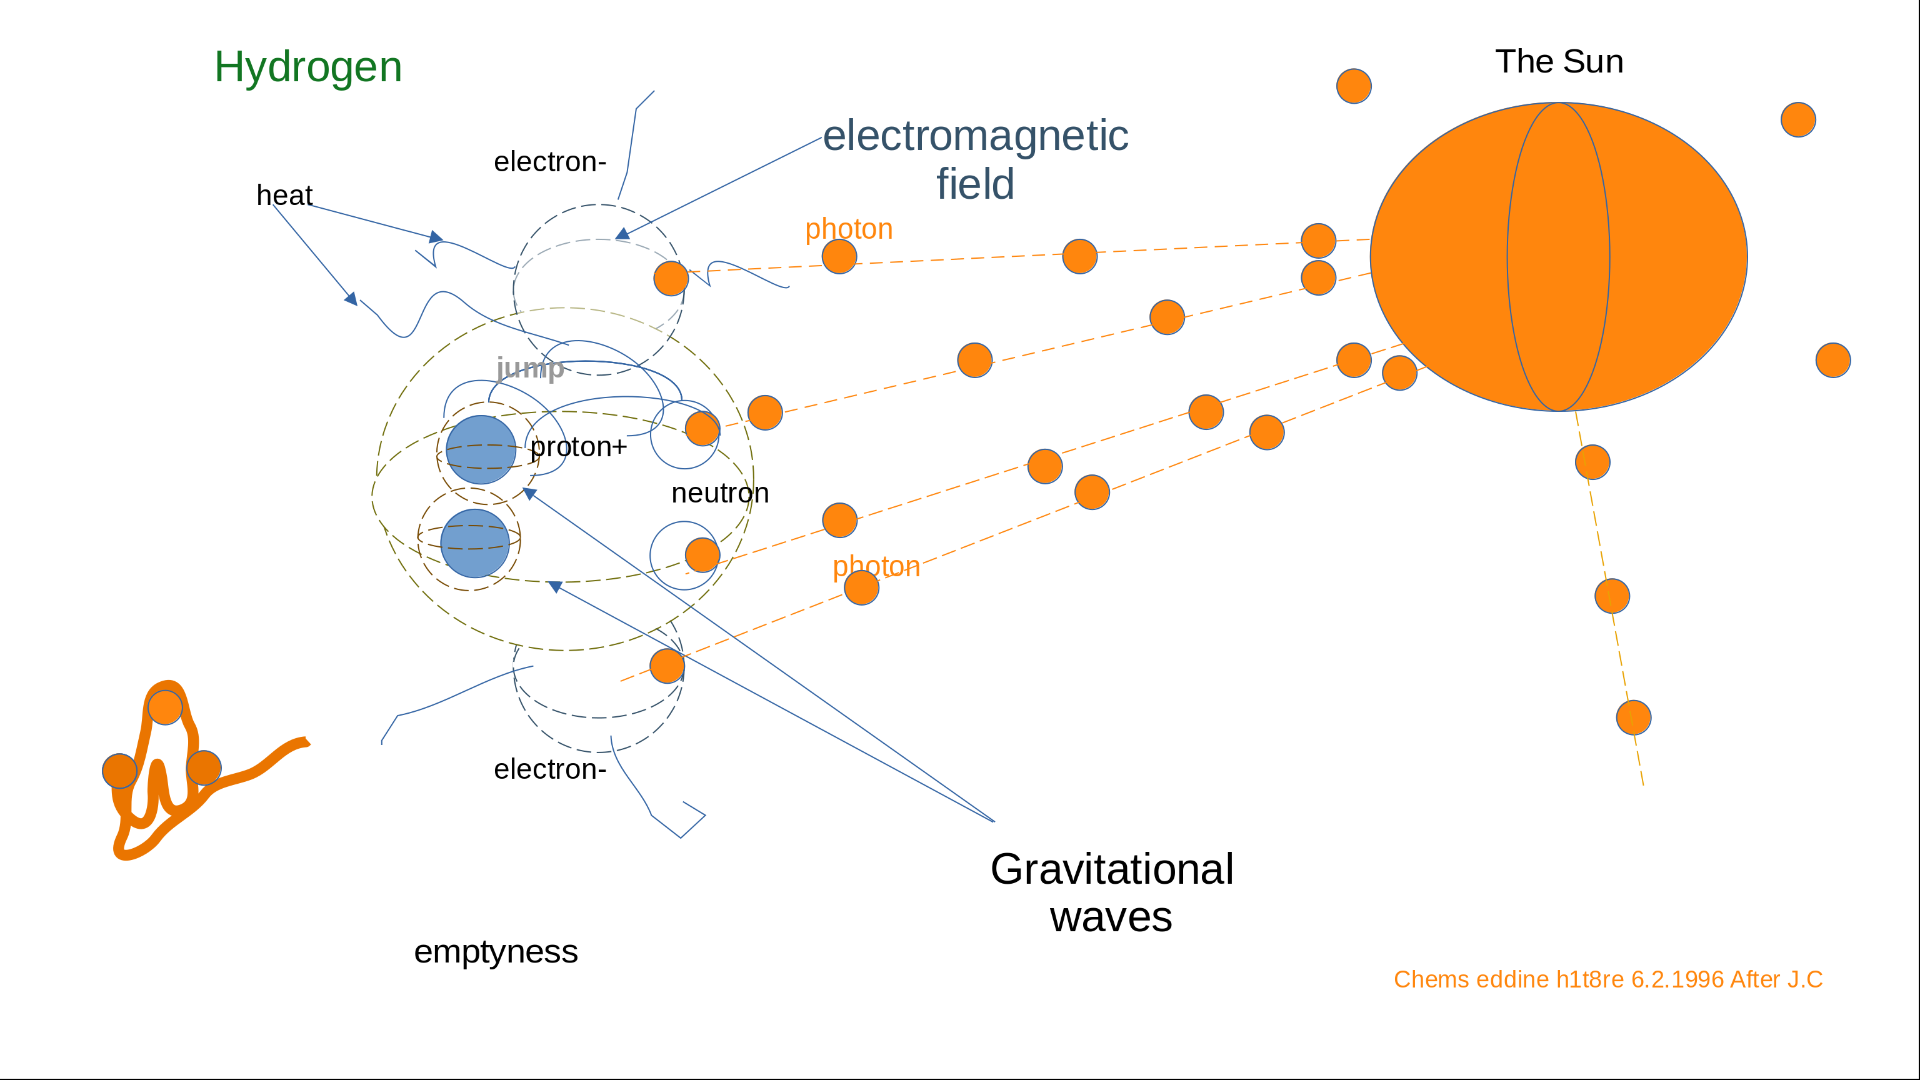
\includegraphics[scale=0.21]{new_science_of_the_world_scheme_by_h1t8re.png}
	\end{center}
	
	`Light coming from the Sun give energy to electron's, forming the grid, and to neutron's charging themself's becoming proton's, by 2, dissolved create a gravitational wave doing with the electromagnetic field of electron's, moving the nucleon of atom through the Univers.
	
	Hydrogen, the simplest atom — one nucleon, one electron — is the perfect witness of the mechanism described in Chapter 2. The scheme of this chapter shows it. On one side, the light coming from the Sun gives energy to the electron's, and these electrons form the grid of light described in 2.1 — the grid going to infinity. On the other side, the same light gives energy to the neutron's, charging themself's, and the neutron's become proton's — this is the condensation of 2.4. Then, by 2 — by pairs, by the duality of the two charges — the proton's are dissolved, and their dissolution creates a gravitational wave. This gravitational wave then works with the electromagnetic field of the electron's: the wave from the center meets the field from the periphery, and their combined action moves the nucleon of the atom through the Univers.
	
	This is the central image of the report: the atom is not a fixed object carried passively through space; it is a small engine. It receives light, it charges its electron's, it condenses and dissolves its nucleon, it emits gravitational waves, it exchanges them with its own electromagnetic field, and by this internal circulation of energie's it propels itself through the Univers. And since hydrogen is the most abundant matter of the universe, what is true for one hydrogen atom is true for the galaxies themselves: the Univers moves because, atom by atom, light, electrons, and gravitational waves are working together in the manner of the scheme.
	
	\newline\newline\newline\newline\newline\newline\newline\newline\newline\newline
	\chapter{Equalities resolution}
	\newline\newline
	The system is resolved with help of two axiom's 
	$\rightarrow$
	\begin{equation}
		$\Longleftrightarrow$
		\left\{ 
		\begin{array}{rcl}
			(f - g)^2' = f'g - 2fg + fg'\\
			\int(1)' = 1 
		\end{array} 
		\right.
	\end{equation}
	\begin{equation}
		$\Longleftrightarrow$
		\left\{ 
		\begin{array}{rcl}
			Energy(Electricity)             &=& Energy(Electromagnetic) \\
			Energy(Electromagnetic) &=& Energy(Gravitational) 
		\end{array} 
		\right.
		\newline\newline\newline\newline
		if : \rho _1 = U and \rho _2 = I\\
		\newline\newline\newline\newline
		$\Longleftrightarrow$
		\left\{ 
		\begin{array}{rcl}
			U.I.$\Delta$T  = \int\int\int\frac{x1.x2}{4.pi. \epsilon_0.||x2-x1||^2}.dx1.dx2 \\
			\int\int\int\frac{x1.x2}{4.pi. \epsilon_0 . ||x2-x1||^2}.dx1.dx2 =\int\int\frac{G.x1.x2}{||x2-x1||^2}.dx1.dx2 
		\end{array} 
		\right.
		\newline\newline\newline\newline
		$\Longleftrightarrow$
		\left\{ 
		\begin{array}{rcl}
			[((U.I)'.$\Delta$T) + U.I.$\Delta$T)]' &=& \int\frac{x1.x2}{4.pi. \epsilon_0.||x2-x1||^2}.dx1.dx2\\
			\frac{(x1'x2+x1x2').||x2-x1||^2 - 2.x1.x2.||x2-x1||}{4.pi.\epsilon_0.||x2-x1||^4} &=& \frac{G.x1.x2}{||x2-x1||^2}
		\end{array}
		\right.
		\newline\newline\newline\newline
		$\Longleftrightarrow$
		\left\{ 
		\begin{array}{rcl}
			[((U.I)'.$\Delta$T) + U.I.$\Delta$T)]' &=&\frac{(U-I)^2'}{4.pi.\epsilon_0.||x2-x1||^2}\\
			\frac{f(||x2-x1||)(U - I)^2'}{(4.pi.\epsilon_0)^2.||x2-x1||.U.I}&=&  G
		\end{array}
		\right.
		\newline\newline\newline\newline
		$\Longleftrightarrow$
		\left\{ 
		\begin{array}{rcl}
			[U.I.$\Delta$T]" &=&\frac{(U-I)^2'}{4.pi.\epsilon_0 . ||x2-x1||^2}\\
			\frac{(U - I)^2'}{4.pi.\epsilon_0.||x2-x1||^4}.\frac{||x2 - x1||^2}{U.I} &=&  G
		\end{array}
		\right.
		\newline\newline\newline\newline
		\begin{equation}
			$\Longleftrightarrow$
			\left\{ 
			\begin{array}{rcl}
				[(U.I+$\Delta$T]^{2''} = \frac{f(||x2-x1||).(U-I)^{2'}}{(4.pi.\epsilon_0)^{2}.||x2-x1||^{3}}\\
				G &=& \frac{f(||x2-x1||)(U - I)^{2'}}{(4.pi.\epsilon_0)^{2}U.I.||x2-x1||}
			\end{array}
			\right.
		\end{equation}
		\newline\newline\newline\newline
		\begin{equation}
			$\Longleftrightarrow$
			\left\{ 
			\begin{array}{rcl}
				G &=& \frac{f(||x2-x1||)(U - I)^{2'}}{(4.pi.\epsilon_0)^{2}U.I.||x2-x1||}\\
				\epsilon_0 &=& \sqrt{ \frac{f(||x2-x1||).(U - I)^{2'}}{[(U.I)+T]^{2''}.(4.pi)^{2}.||x2-x1||^{3}}
				\end{array}
				\right.
			\end{equation}
			\newline\newline\newline\newline
			The result of this equality:
			\begin{equation}
					Energy(Electromagnetic) &=& Energy(Gravitational)
					\Rightarrow
			\end{equation}
			With the resolution of the system: 
			\newline\newline\newline\newline
			\begin{equation}
				\Rightarrow
				\int\int\frac{G.x1.x2}{||x2-x1||^2}.dx1.dx2 = \int\int\int\frac{x1.x2}{4.pi. \epsilon_0 . ||x2-x1||^2}.dx1.dx2
			\end{equation}
				the result is:
				\newline\newline\newline\newline
			\begin{equation}
				G &=& \frac{f(||x2-x1||)(U - I)^{2'}}{(4.pi.\epsilon_0)^{2}U.I.||x2-x1||}\\
				|
				| 
				\epsilon_0 &=& \sqrt{ \frac{f(||x2-x1||).(U - I)^{2'}}{[(U.I)+T]^{2''}.(4.pi)^{2}.||x2-x1||^{3}}
			\end{equation}
					
				
			\begin{equation}
					\newline\newline\newline\newline
					k0 = f(distance)
					\newline\newline\newline\newline
					k1 = f(distance)
					\newline\newline\newline\newline
				\end{equation}			
				
				The method deserves a word of explanation. The two axiom's are the tools that allow the passage from the integral form to the derivative form: the first axiom gives the rule for the derivative of a squared difference of two functions, the second gives the integral of a derivative. With them, the triple and double integrals of the electromagnetic and gravitational energies can be unfolded, step by step, into expressions where only U, I, T, and the distance ‖x2−x1‖ remain. Each step of the chain above is one unfolding: the electricity U·I·ΔT is derived, the integral of the electromagnetic field is reduced, and the two members of each equality are progressively put in comparable forms, until G and ε0 appear isolated on one side. This is the resolution proper: the system is not solved for x1 and x2, it is solved for the constants G and ε0, which are the hidden variables of the world.
				
				**Interpretation of G.** We can say that it's the grid going from the Sun to Infinity. It can be The Sun and the Blackhole doing the Galaxy moving in space, starting from the bigbang. The Sun is giving photon's for electron's of the grid; charging; interacting with gravitation through the electro-magnetic field. With the grid photon's can be seen like a particule and can be seen like a wave. By this equalities we gonna describe the gravitational constant G and describe ε0 the permettivity of matter to go through empytness.
				
				**The gravitational constant G is tension minus current variating by themself's by a distance on two electromagnetic sphere's with power.** This sentence must be read literally. G, the constant that classical engineering treats as a fixed universal number, is here re-expressed as a relation between tension U, current I, their variations (U−I)²′, the power U·I, and the distance ‖x2−x1‖ between two electromagnetic sphere's. G is therefore not a dead constant: it is the signature of the live exchange between two charged sphere's — for example the Sun and the Blackhole — doing the Galaxy moving in space. The two functions of distance, k0 = f(distance) and k1 = f(distance), encode how this exchange weakens or strengthens with the separation of the sphere's. And with the grid, the photon's can be seen like a particule and can be seen like a wave — the grid resolves the old duality: light is both, because the grid is made of units (particule's) that extend to infinity (wave).
				
				It's the nucleon of the atom liffing with the grid of electron's. The proton's of the atom dissolving themself's creating a gravitational wave working with electron's of the grid and become neutron's charged with photon's being proton's. Here the cycle is closed and it must be read slowly, because it is the engine of the universe in one sentence: the proton's dissolve themselves, creating a gravitational wave; this wave works with the electron's of the grid; the neutron's are charged with photon's and become proton's again; and the cycle restarts. Condensation, dissipation, wave, charge, condensation again — the eternal return of the energie's, described in Chapter 2 at the scale of one atom, is here the same mechanism that moves the Galaxy.
				
				**Interpretation of ε0.** ε0 is permittivity of matter to go through emptyness. It's racine of tension minus current variating by themself's by two sphere's on power with time accelerating on three dimension's. The permittivity is thus not an inert property of the vacuum: it is the root of the same live exchange — tension minus current variating by themself's, on two sphere's, on power, with time accelerating, on three dimension's. The three dimension's of the triple integral of Chapter 1 are still there, in the ‖x2−x1‖³ of the denominator: emptyness permits matter to pass only by occupying its three dimensions in time.
				
				
				The resolution continues to light itself. The same method applies to the equality with the energy of light:
				\newline\newline\newline\newline
			\begin{equation}\
				\begin{array}{rcl}
					\newline\newline
					m*C^{2}  &=& \int\int\int\frac{x1.x2}{4.pi. \epsilon_0 ||x2-x1||^2}.dx1.dx2\\
					\Rightarrow
					\newline\newline
					m*C^{2}  &=& \int\int\frac{(U'.I+U.I').||x2-x1||^{2}-2.U.I.||x2-x1||}{(4.pi.\epsilon_0 )^{2}. ||x2-x1||^{4}}.dx1.dx2\\
					\Rightarrow
					m*C^{2}  &=& \int\int\frac{f(||x2-x1||.(U-I)^{2'}}{(4.pi. \epsilon_0 )^{2}. ||x2-x1||^{4}}.dx1.dx2\\
					\newline\newline
				\end{array}
			\end{equation}
				\newline\newline
				This last system can be life going through the Univers..
				\newline\newline\newline\newline
				The conclusion is:
				\newline\newline
				With the equality $E_{light} = E_{electrical}$
				\newline\newline
				$C = \sqrt{\frac{U.I.T}{m}}$ ==> $\frac{km}{s^{2}}.\frac{km.kg}{s} = V.A$
				\newline\newline
				We know that **P(ower) = V·A**. This mean that **power is acceleration of speed of matter**. This first conclusion already inverts the habitual reading of engineering. Power is not an abstract quantity invoiced on a bill; it is, physically, an acceleration of speed of matter. Every watt delivered by a circuit, every volt-ampere passing in a wire, is matter being accelerated — the same acceleration that the nucleon's feel when the gravitational waves push them through the Univers. The equality C = √(U·I·T/m) makes it explicit: the speed of light itself, squared, is tension times current times time divided by mass. Light, electricity, and matter are one.
				
				We know that $P_{ower} = V.A$
				\newline\newline
				This mean that power is acceleration of speed of matter..
				\newline\newline
				With the equality $E_{gravitational} = E_{electromagnetic}$
				\newline\newline
				$\frac{ f(||x2-x1||).(U-I)^{2'}. }{ (4.pi)^{2}.U.I.||x2-x1||.\frac{f(||x2-x1||).(U-I)^{2'}}{((U.I)+T)^{2"}.(4.pi)^{2}.||x2-x1||^{3}}} = \int_a^b \frac{U.I}{4.pi.\frac{f(||x2-x1||).(U-I)^{2'}}{((U.I)+T)^{2"}.(4.pi)^{2}.||x2-x1||^{3}}}$
				\newline\newline
				After resolution of the equality we find that:
				\newline\newline
				$P_{ower} = U.I = \frac{f(||x2-x1||).(U-I)^{'}}{((U.I)+T)^{"}}$
				\newline\newline
				The last equality mean that **power is tension minus current variating on power plus time accelerating**.
				
				Here is the final sentence of the resolution, and it unifies everything. Power, U·I, which was already acceleration of speed of matter, is now also tension minus current variating — the same (U−I) that appears inside G and inside E0 — on power plus time accelerating — the same (U·I + T) that carries the second derivative ″, the acceleration. All the threads of the report meet in this single line: the (U−I) of the gravitational constant, the time of the electrical energy, the acceleration of the conclusion, the power that is both tension·current and tension-current variating on tension.current plus time accelerating. The world described by this report is therefore complete: a grid of light going from the Sun to infinity, charged electrons forming the channels of electricity, nucleon's condensing and dissolving into gravitational waves, an electromagnetic field connecting everything through the three dimensions of emptyness, and one single currency — power — converting itself without rest between all these forms, moving the atom's, moving the galaxies, and making life going through the Univers. This is the description of the world by engineering of energie's. And at first, the purpose remains: to get fly my pyramid's Shoon|Eachbe.
				
			\end{document}